\documentclass[fleqn, 12pt]{article}
% Packages
\usepackage[0.9, font.kp, swapVarGreek]{sigilz}
\usepackage{hyperref}
\usepackage{url}

\usepackage{listings}
\usepackage{color}

\definecolor{dkgreen}{rgb}{0,0.6,0}
\definecolor{gray}{rgb}{0.5,0.5,0.5}
\definecolor{mauve}{rgb}{0.58,0,0.82}
\lstset{frame=tb,
  aboveskip=3mm,
  belowskip=3mm,
  showstringspaces=false,
  columns=flexible,
  basicstyle={\small\ttfamily},
  keywordstyle=\color{blue},
  commentstyle=\color{dkgreen},
  stringstyle=\color{mauve},
  breaklines=true,
  breakatwhitespace=true,
  tabsize=3
}

% Header
\setlength{\headheight}{15pt}
\pagestyle{fancy}
\lhead{Adam B Jones and Fei Yuan}
\chead{PHY982}
\marginparsep=2cm

% Environments
\definecolor{correctioncolor}{rgb}{.7, .2, 0}
\provideenvironment{correction}{\begingroup\color{correctioncolor}}{\endgroup}
\provideenvironment{valigntop}%
{\begin{minipage}[t]{\textwidth}\vspace{0pt}}%
{\vspace{0pt}\end{minipage}}

% Commands
\providecommand{\Dom}{\operatorname{Dom}}
\providecommand{\Roots}{\operatorname{Roots}}
\providecommand{\pvint}{\fint}
\providecommand{\integral}{\mathop{\textstyle\int}}
\providecommand{\ointegral}{\mathop{\textstyle\oint}}
\def\oint{\ointctrclockwise}

% note: \textcolor for fg; \colorbox for bg
\definecolor{rescolor}{rgb}{.8, .9, 1}
\newcommand{\resmath}[1]{\colorbox{rescolor}{\ensuremath{\displaystyle
      #1}}}

\rhead{HW3}
\begin{document}

\begin{enumerate}

\item \part*{Derive the transformation from CM to Lab cross sections.}

\begin{figure}
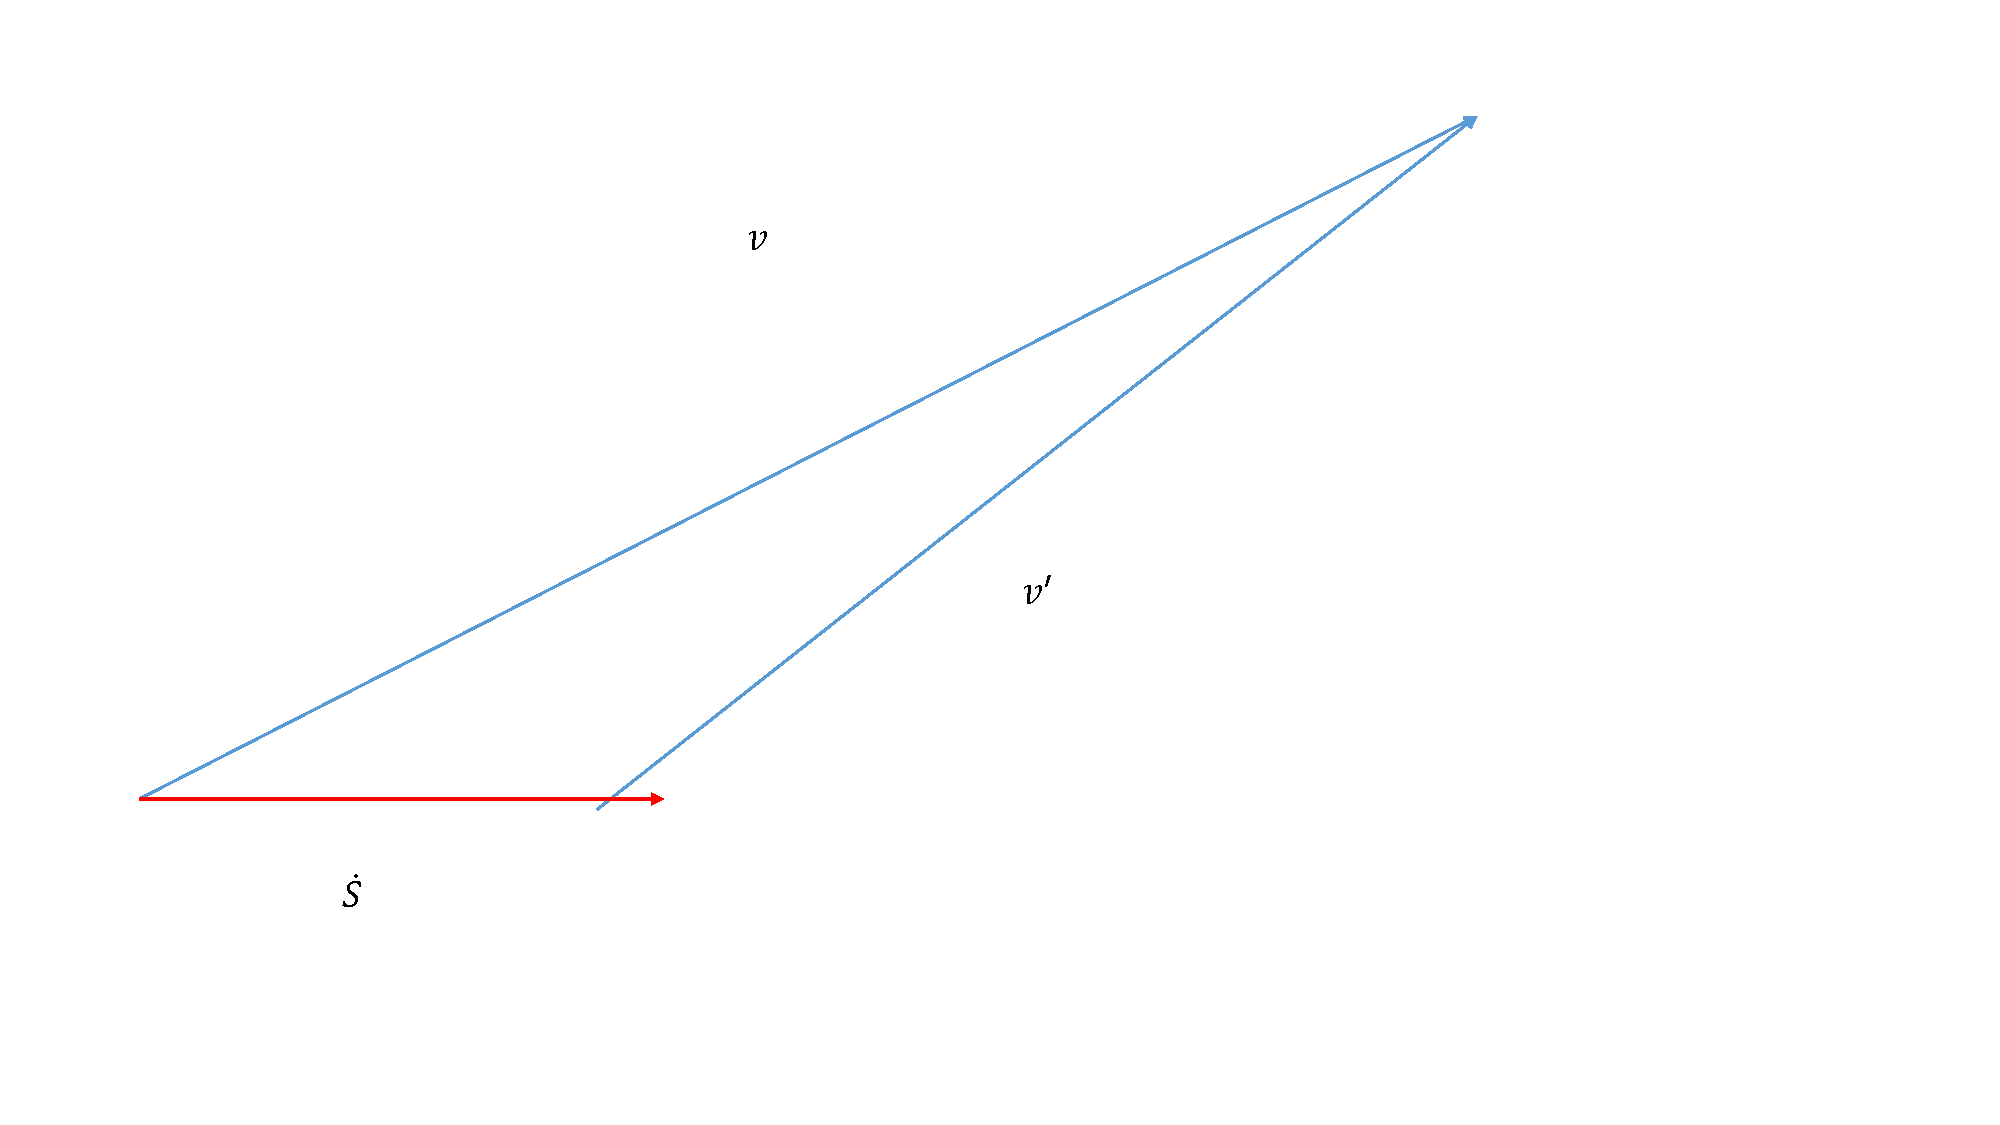
\includegraphics[width=0.8\textwidth]{hw3-comlab.pdf}\protect\caption{The relation between CM and Lab frames.}
\end{figure}


The relation ship between the center of mass and lab velocites is
given by the following equations and can be seen in the figure:

\begin{eqnarray*}
v{}_{c}^{\prime}\sin\theta=v_{c}\sin\theta_{lab} & \dot{S}+v_{c}^{\prime}\cos\theta=v_{c}\cos\theta_{lab} & \phi=\phi_{lab}\\
 & \vec{v_{c}}=\vec{v_{c}^{\prime}}+\dot{\vec{S}}
\end{eqnarray*}


The parameter $\rho$ is defined as: $\rho\equiv\frac{\dot{S}}{v_{c}'}$.
The relationship between the lab and cm scattering angle can be expessed
as: $\tan\theta_{lab}=\frac{\sin\theta}{\rho+\cos\theta}$. We also
know that conservation of flux requires the scattering crossection
of an infinitessimal solid angle is conseerved by the chang of referance
frame. This leads to the following expressison:

\[
\sigma_{lab}(\theta_{lab},\phi_{lab})d\phi_{lab}\sin\theta_{lab}d\theta_{lab}=\sigma(\theta.\phi)d\phi\sin\theta d\theta\Rightarrow\sigma_{lab}(\theta_{lab},\phi_{lab})=\sigma(\theta,\phi)\frac{d\phi}{d\phi_{lab}}\frac{\sin\theta}{\sin\theta_{lab}}\frac{d\theta}{d\theta_{lab}}
\]


Clearly$\frac{d\phi}{d\phi_{lab}}=1$ and:

\[
\frac{\sin\theta}{\sin\theta_{lab}}=\frac{v_{c}}{v_{c}^{\prime}}=\frac{\sqrt{\vec{v_{c}}\centerdot\vec{v_{c}}}}{v'}=\frac{\sqrt{v_{c}^{2}+2v_{c}\dot{S}\cos\theta+\dot{S}^{2}}}{v'}=\sqrt{1+2\rho\cos\theta+\rho^{2}}
\]


To find the the derivative of $\theta$:

\[
\frac{d}{d\theta_{lab}}\left(\tan\theta_{lab}\right)=\frac{d}{d\theta_{lab}}\left(\frac{\sin\theta}{\rho+\cos\theta}\right)
\]


\[
\sec^{2}\theta_{lab}=\frac{1+\rho\cos\theta}{\left(\rho+\cos\theta\right)^{2}}\frac{d\theta}{d\theta_{lab}}
\]


\[
\Rightarrow\frac{d\theta}{d\theta_{lab}}=\cos^{2}\theta_{lab}\left(\frac{1+\rho\cos\theta}{\left(\rho+\cos\theta\right)^{2}}\right)
\]


But:

\[
\cos^{2}\theta_{lab}=\left(\frac{\dot{S+v_{c}^{\prime}\cos\theta}}{v_{c}}\right)^{2}=\left(\frac{v_{c}^{\prime}}{v_{c}}\right)^{2}\left(\rho+\cos\theta\right)^{2}\Rightarrow\frac{d\theta}{d\theta_{lab}}=\left(\frac{v_{c}^{\prime}}{v_{c}}\right)^{2}\left(1+\rho\cos\theta\right)
\]


So we have:

\[
\sigma_{lab}\left(\theta,\phi\right)=\sigma(\theta,\phi)\left(\frac{v_{c}^{\prime}}{v_{c}}\right)^{3}\frac{1}{1+\rho\cos\theta}=\sigma(\theta,\phi)\frac{\left(1+2\rho\cos\theta+\rho^{2}\right)^{3/2}}{1+\rho\cos\theta}
\]
 QED.

\item Assume we have a short-ranged, spherically symmetric potential $V(r)$.
  The incident beam is a plane wave of momentum of $k$ originating from the
  negative z-axis:
  \begin{align*}
    \psi_{\text i}(\bm r) = \E^{\I k z}
  \end{align*}
  The scattered wave has the asymptotic form
  \begin{align*}
    \psi_{\text f}(\bm r) = f(\theta) \frac{\E^{\I k r}}{r}
  \end{align*}
  where we have omitted the azimuth $\phi$ due to symmetry.

  The Schr\"odinger equation of this problem is:
  \begin{align*}
    \left(-\frac{\hbar^2}{2 m} \nabla^2 + V(r)\right) \psi(\bm r)
    = E \psi(\bm r)
  \end{align*}
  In spherical coordinates, the Laplacian is given by:
  \begin{align*}
  -\nabla^2 = \frac{1}{r^2} (\hat \ell^2 - \frac{\D}{\D r} r^2 \frac{\D}{\D r})
  \end{align*}
  where $\hat{\bm \ell}$ is the orbital angular momentum operator, whose
  eigenvalues are of the form $\ell (\ell + 1)$.  Due to azimuthal symmetry,
  the only possible angular eigenstates are the ones with $m = 0$, which are
  simply the Legendre polynomials composed with cosine: $P_\ell(\cos \theta)$.

  Hence, we shall expand the incoming wave as a sum of Legendre polynomials:
  \begin{align*}
    \E^{\I k z} =
    \sum_{\ell = 0}^\infty a_\ell P_\ell(\cos \theta)
  \end{align*}
  To do this, we use the orthogonality relations
  \begin{align*}
     \int_0^\PI P_\ell(\cos \theta) P_{\ell'}(\cos \theta) \sin \theta \D \theta
    = \frac{2}{2 \ell + 1} \Kroneckerdelta_{\ell \ell'}
  \end{align*}
  to obtain the coefficients:
  \begin{align*}
     \frac{2}{2 \ell + 1} a_\ell
    = \int_0^\PI P_\ell(\cos \theta) \E^{\I k r \cos \theta} \sin \theta \D \theta
  \end{align*}
  According to NIST 10.54.3 (\url{http://dlmf.nist.gov/10.54#E2}), this
  integral is proportional to the spherical Bessel function:
  \begin{align*}
    \dots = \frac{2}{(-\I)^\ell} j_\ell(k r)
  \end{align*}
  Thus,
  \begin{align*}
    \E^{\I k z} =
    \sum_{\ell = 0}^\infty (2 \ell + 1) \I^\ell j_\ell(k r) P_\ell(\cos \theta)
  \end{align*}
  The spherical Bessel functions $j_\ell$ (regular) and $y_\ell$ (irregular)
  are related to the Riccati--Hankel functions $\zeta_\ell$ (incoming) and
  $\xi_\ell$ (outgoing) by:
  \begin{align*}
    &\zeta_\ell(s) = s (j_\ell(s) - \I y_\ell(s)) \\
    &\xi_\ell(s) = s (j_\ell(s) + \I y_\ell(s))
  \end{align*}
  Therefore, the plane waves may also be written as:
  \begin{align*}
    \E^{\I k z} =
    \sum_{\ell = 0}^\infty (2 \ell + 1) \I^\ell
    \frac{1}{2 k r} (\zeta_\ell(k r) + \xi_\ell(k r)) P_\ell(\cos \theta)
  \end{align*}
  In this form, the partial wave S-matrix element $S_\ell$ is defined as the
  coefficient of the outgoing wave in the asymptotic wave function:
  \begin{align*}
    \psi(\bm r) \sim \sum_{\ell = 0}^\infty (2 \ell + 1) \I^\ell
    \frac{1}{2 k r} (\zeta_\ell(k r) + S_\ell \xi_\ell(k r)) P_\ell(\cos \theta)
  \end{align*}
  The incoming wave must have the same coefficient as that of the plane wave
  due to the boundary conditions.

  The scattered wave $\psi_{\text f}$ is the difference between the full wave
  function $\psi$ and the incident plane wave $\psi_{\text i}$, hence its
  asymptotic form is also their respective difference:
  \begin{align*}
    \psi_{\text f}(\bm r) \sim \sum_{\ell = 0}^\infty (2 \ell + 1) \I^\ell
    \frac{1}{2 k r} (S_\ell - 1) \xi_\ell(k r) P_\ell(\cos \theta)
  \end{align*}
  We can factor out the spherical wave
  \begin{align*}
    \psi_{\text f}(\bm r) \sim \frac{\E^{\I k r}}{r}
    \sum_{\ell = 0}^\infty (2 \ell + 1) \I^\ell
    \frac{1}{2 k} (S_\ell - 1) \frac{\xi_\ell(k r)}{\E^{\I k r}} P_\ell(\cos \theta)
  \end{align*}
  and use the asymptotic behavior of the Riccati--Hankel functions
  \begin{align*}
    \xi_\ell(s) \sim \I^{-(\ell + 1)} \E^{\I s}
  \end{align*}
  to simplify the result for large $r$:
  \begin{align*}
    \psi_{\text f}(\bm r)
    &\sim \frac{\E^{\I k r}}{r}
    \sum_{\ell = 0}^\infty (2 \ell + 1) \I^\ell
    \frac{1}{2 k} (S_\ell - 1) \I^{-(\ell + 1)} P_\ell(\cos \theta) \\
    &=\frac{\E^{\I k r}}{r}
    \frac{1}{2 \I k} \sum_{\ell = 0}^\infty (2 \ell + 1)
    P_\ell(\cos \theta) (S_\ell - 1)
  \end{align*}
  From this, we may read off the scattering amplitude $f$:
  \begin{align*}
    f(\theta) =
    \frac{1}{2 \I k} \sum_{\ell = 0}^\infty (2 \ell + 1)
    P_\ell(\cos \theta) (S_\ell - 1)
  \end{align*}

\item Starting witht the relationship between cross section and scattering
length we can use the result of problem 2.

\begin{eqnarray*}
\sigma_{el}\left(\theta\right) & =|f(\theta)|^{2} & =\left\Vert \frac{1}{2\boldsymbol{i}k}\right\Vert ^{2}\left\Vert \sum_{L=0}^{\infty}\left(2L+1\right)P_{L}\left(\cos\theta\right)\left(S_{L}-1\right)\right\Vert ^{2}\\
 &  & {\displaystyle =\frac{1}{4k^{2}}\sum_{L,L^{\prime}=0}^{\infty}\left(2L+1\right)P_{L}\left(\cos\theta\right)\left(S_{L}-1\right)\left(2L^{\prime}+1\right)P_{L}^{*}\left(\cos\theta\right)\left(S_{L^{\prime}}^{*}-1\right)}
\end{eqnarray*}


Using the normalization condition for the Legendre polynomial $\int_{-1}^{+1}P_{L^{\prime}}^{*}(x)P_{L}(x)dx=\frac{2\delta_{LL^{\prime}}}{2L+1}$:

\begin{eqnarray*}
\int_{0}^{2\pi}d\phi\int_{0}^{\pi}d\theta\sigma_{el}\left(\theta\right) & =\frac{\int_{0}^{2\pi}d\phi}{4k^{2}}\sum_{L,L^{\prime}=0}^{\infty}\left(2L+1\right)\left(2L^{\prime}+1\right)\left(S_{L}-1\right)\left(S_{L^{\prime}}^{*}-1\right))\int_{0}^{\pi}P_{L}\left(\cos\theta\right)P_{L}^{*}\left(\cos\theta\right)d\theta\\
 & =\frac{2\pi}{4k^{2}}\sum_{L,L^{\prime}=0}^{\infty}\left(2L+1\right)\left(2L^{\prime}+1\right)\left(S_{L}-1\right)\left(S_{L^{\prime}}^{*}-1\right)\frac{2\delta_{LL^{\prime}}}{2L+1}
\end{eqnarray*}


Evaluating the sum over $L^{\prime}$yields:

\[
\sigma_{el}==\frac{\pi}{k^{2}}\sum_{L=0}^{\infty}\left(2L+1\right)\left(\|S_{L}\|^{2}-\left(S_{L}+S_{L}^{*}\right)+1\right)=\frac{2\pi}{k^{2}}\sum_{L=0}^{\infty}\left(2L+1\right)\left(1-Re(S_{L})\right)
\]


Where I have used the fact that $\|S_{L}\|^{2}=1$in the case of elastic
scattering. We can write $S_{L}=\exp(\mathbf{i}\phi)\Rightarrow\log(S_{L})=i\phi$
let $\delta_{L}=\frac{\log(S_{L})}{2\mathbf{i}}+N(E)\pi=\frac{\phi}{2}$
be the regularized phase shift. This implies $Re(S_{L})=\cos\phi=\cos^{2}\frac{\phi}{2}-\sin^{2}\frac{\phi}{2}$
therefore we have:

\[
\sigma_{el}=\frac{2\pi}{k^{2}}\sum_{L=0}^{\infty}\left(2L+1\right)\left(1-\left(\cos^{2}\delta_{L}-\sin^{2}\delta_{L}\right)\right)=\frac{4\pi}{k^{2}}\sum_{L=0}^{\infty}\left(2L+1\right)\sin^{2}\delta_{L}
\]


QED.

\item Assuming a phase shift around a resonance with the usual shape:
  \begin{align*}
    \delta(E) = \delta_{\text{bg}}(E) +
    \operatorname{atan2}\left(\frac{\Gamma}{2}, E_{\text r} - E\right)
  \end{align*}
  The S-matrix element can be recovered by exponentiation:
  \begin{align*}
    S(E)
    &= \left(\E^{\I \delta(E)}\right)^2 \\
    &= \left(\E^{\I \delta_{\text{bg}}(E)}
      \E^{\I \operatorname{atan2}(\Gamma / 2, E_{\text r} - E)}\right)^2
  \end{align*}
  The arguments of $\operatorname{atan2}$ may be interpreted as the phase of a
  complex number with unit magnitude:
  \begin{align*}
    \frac{\I \Gamma / 2 + E_{\text r} - E}{
    |\I \Gamma / 2 + E_{\text r} - E|}
  \end{align*}
  Allowing the exponentiation to cancel the effect of $\operatorname{atan2}$:
  \begin{align*}
    S(E)
    &= \left(\E^{\I \delta(E)}\right)^2 \\
    &= \left(\E^{\I \delta_{\text{bg}}(E)}
      \frac{\I \Gamma / 2 + E_{\text r} - E}{
      |\I \Gamma / 2 + E_{\text r} - E|}\right)^2 \\
    &= \E^{2 \I \delta_{\text{bg}}(E)}
      \frac{(\I \Gamma / 2 + E_{\text r} - E)^2}{
      |\I \Gamma / 2 + E_{\text r} - E|^2} \\
    &= \E^{2 \I \delta_{\text{bg}}(E)}
      \frac{\I \Gamma / 2 + E_{\text r} - E}{
      -\I \Gamma / 2 + E_{\text r} - E} \\
    &= \E^{2 \I \delta_{\text{bg}}(E)}
      \frac{E - E_{\text r} - \I \Gamma / 2}{
      E - E_{\text r} + \I \Gamma / 2}
  \end{align*}
  It is evident from this equation that the S-matrix element is singular when
  $E = E_{\text r} + \I \Gamma / 2$.  In particular, it is a simple pole that,
  when expanded to first order, has the general form above.

  In the complex energy plane, there exists an eigenstate of the Schr\"odinger
  equation with a complex energy of $E_{\text r} + \I \Gamma / 2$.  One can
  infer that it is resonance state because it has a finite lifetime:
  \begin{align*}
    \Psi(\bm r; t) \propto \E^{\I (E_{\text r} + \I \Gamma / 2) t / \hbar}
    = \E^{\I E_{\text r} t / \hbar} \E^{-\Gamma t / (2 \hbar)}
  \end{align*}

\item Starting from Fermi's golden rule we have:

\[
dJ=\|M_{fi}\|^{2}dN_{f}2\pi\delta\left(E_{f}-E_{i}\right)
\]


Free particles compose our initial and final states:

\[
{\displaystyle |\Psi_{i(f)}>}=\frac{1}{\sqrt{V}}\exp\left(\mathbf{i}\vec{p_{f(i)}}\centerdot\vec{r}\right)\Rightarrow M_{fi}=<\Psi_{f}|U(\vec{r})|\Psi_{i}>=\frac{1}{V}\int\exp\left(\mathbf{i}\vec{p_{f}}\centerdot\vec{r}\right)U(x)\exp\left(\mathbf{i}\vec{p_{i}}\centerdot\vec{r}\right)d^{3}r
\]


Where $V$ is an arbitrary normalization factor. Since we are interested
in the Coulomb potential of a nucleus with atomic number Z we have
$U(\vec{r})=\frac{Z_{1}Z_{2}\alpha}{r}$thus:

\[
M_{fi}=\frac{1}{V}\int\exp\left(\mathbf{i}\vec{q}\centerdot\vec{r}\right)\frac{Z_{1}Z_{2}\alpha}{r}d^{3}r=\frac{Z_{1}Z_{2}\alpha}{V}\frac{4\pi}{q^{2}}
\]


Where I have used the definition of the momentum transfer $\vec{q}=\vec{p_{f}}-\vec{p_{i}}$and
the 3-d Fourier trasnsform of the Coulomb potential $\mathcal{F}(\frac{1}{r})=\frac{4\pi}{k^{2}}$.

We can use the cannonical relationship between particle current and
cross section: $dJ=jNd\sigma$ where $j$ is the magnitude of the
probability current given by:

\[
\vec{j}=\frac{\hbar}{2m\mathbf{i}}\left(\Psi^{*}\nabla\Psi-\Psi\nabla\Psi^{*}\right)=\frac{\hbar\vec{p}}{mV}=\frac{\hbar\vec{v}}{V}
\]


So the cross section is:

\[
d\sigma=\frac{dJ}{j_{i}N}=\frac{\|M_{fi}\|^{2}V}{4\pi^{2}v_{i}}d^{3}p_{f}\delta\left(E_{f}-E_{i}\right)
\]


Using $d^{3}p_{f}=p_{f}^{2}dp_{f}d\Omega$ and integrating our equation
to enforce energy conservation:

\[
\frac{d\sigma}{d\Omega}=\frac{\|M_{fi}\|^{2}V}{4\pi^{2}v_{i}}\int dp_{f}p_{f}^{2}\delta(E_{f}-E_{i})=\frac{\|M_{fi}\|^{2}V}{4\pi^{2}v_{i}}\int\frac{dp_{f}}{dE_{f}}dE{}_{f}p_{f}^{2}\delta(E_{f}-E_{i})
\]


\[
=\frac{\|M_{fi}\|^{2}Vp_{f}^{2}}{4\pi^{2}v_{i}v_{f}}=\frac{4\left(Z_{1}Z_{2}\right)^{2}\alpha^{2}p_{f}^{2}}{q^{4}v_{i}v_{f}}
\]


Since our colision is eleastic we have $p_{f}=p_{i}=p$so $\vec{q}^{2}=\left(\vec{p_{f}}-\vec{p_{i}}\right)^{2}=4p^{2}\sin^{2}\frac{\theta}{2}$
substituting:

\[
\frac{d\sigma}{d\Omega}=\frac{4\left(Z_{1}Z_{2}\right)^{2}\alpha^{2}p^{2}}{16p^{4}\sin^{4}\frac{\theta}{2}v_{i}v_{f}}=\frac{\left(Z_{1}Z_{2}\right)^{2}\alpha^{2}}{4\hbar^{2}k^{2}\sin^{4}\frac{\theta}{2}v^{2}}=\frac{\left(Z_{1}Z_{2}\right)^{2}\alpha^{2}\mu}{4\hbar^{2}k^{2}\sin^{4}\frac{\theta}{2}2E}=\frac{\eta^{2}}{4k^{2}\sin^{4}\frac{\theta}{2}}
\]


Where $\eta=\frac{Z_{1}Z_{2}e^{2}}{\hbar}\left(\frac{\mu}{2E}\right)^{1/2}$
is the Sommerfield parameter.

\item %6

\item It is useful to assert some form of the non-unique \emph{wave operator}
defined by the relationship$\Omega|\Phi_{0}>\equiv|\Psi_{0}>$ where
$|\Phi_{0}>$is some reference state and $|\Psi_{0}>$ is the exact
ground state wave function. We want a form that is \emph{consistent}
\emph{with the Schroedinger equation} (SE). I will choose the form
used in RSPT $\Omega=P+R_{H}HP$ where $R_{H}\equiv Q\left(P+Q\left(E-H\right)Q\right)^{-1}Q=\left(E-QHQ\right)^{-1}Q=Q\left(E-QHQ\right)^{-1}=QR_{H}=R_{H}Q$
is the reduced resolvent of the $H$. Note that $P$ and $Q$ are
projection operators where $P=|\Phi_{0}><\Phi_{0}|$ and $Q$ is its
orthogonal complement. Now to show this wave operator is consistent
with the SE :

\begin{flushleft}
\begin{eqnarray*}
 & \left(E-H\right)|\Psi_{0}>=(P+Q)\left(E-H\right)|\Psi_{0}>\\
 & =P\left(E-H\right)|\Psi_{0}>+Q\left(E-H\right)|\Psi_{0}>\\
 & =P\left(E-H\right)|\Psi_{0}>+Q\left(E-H\right)\Omega|\Phi_{0}>\\
 & =P\left(E-H\right)|\Psi_{0}>+Q\left(E-H\right)\left(P+R_{H}HP\right)|\Phi_{0}>\\
 & =P\left(E-H\right)|\Psi_{0}>+Q\left(E-H\right)\left(|\Phi_{0}>+R_{H}H|\Phi_{0}>\right)\\
 & =P\left(E-H\right)|\Psi_{0}>+Q\left(E-H\right)P|\Phi_{0}>+Q\left(E-H\right)\left(E-H\right)^{-1}QH|\Phi_{0}>\\
 & =P\left(E-H\right)|\Psi_{0}>+Q\left(E-H\right)|\Phi_{0}>+QH|\Phi_{0}>\\
 & =P\left(E-H\right)|\Psi_{0}>=|\Phi_{0}><\Phi_{0}\left(E-H\right)|\Psi_{0}>=0
\end{eqnarray*}

\par\end{flushleft}

Therefore this form of the wave operator is consistent with the SE.
Now we will use the wave operator to derive the form of the effective
Hamiltonian starting from the SE:

\[
\left(E-H\right)|\Psi>=E|\Psi>-H\Omega|\Phi_{0}>=E|\Psi>-H\left(P+R_{H}HP\right)|\Phi_{0}>
\]


\[
=E|\Psi>-H\left(P+QR_{H}QHP\right)|\Phi_{0}>=E|\Psi>-H\left(P+Q(E-QHQ)^{-1}QHP\right)|\Phi_{0}>
\]


Multiplying by $P$ on the left:

\[
\Rightarrow PE|\Psi>-PH\left(P+Q(E-QHQ)^{-1}QHP\right)|\Phi_{0}>
\]


\[
=E|\Phi_{0}>-(PHP+PHQ(E-QHQ)^{-1}QHP)|\Phi_{0}>=\left(E-H_{eff}\right)|\Phi_{0}>=0
\]


We identify the effective Hamiltonian as desired:

\[
H_{eff}=PHP+PHQ(E-QHQ)^{-1}QHP
\]


The optical potential is derived by splitting the Hamiltonian into
teh following pieces $H=T_{0}+H_{A}+V$ where $H_{A}$ is the Hamiltonia
that describes the internal degrees of freedom in the target. Note
that because $E_{0}\equiv0$ that$H_{A}|\Phi_{0}>=0\Rightarrow H_{A}P=PH_{A}=0$
and $PT_{0}=T_{0}|\Phi_{0}>$since $|\Phi_{0}>$does not depend on
the projectile degrees of freedom. So we can write the effective Hamiltonian
as:

\[
H_{eff}=P\left(T_{0}+H_{A}+V\right)P+P\left(T_{0}+H_{A}+V\right)Q(E-QHQ)^{-1}Q\left(T_{0}+H_{A}+V\right)P
\]


\[
=P\left(T_{0}+V\right)P+PVQ(E-QHQ)^{-1}QVP
\]


\[
=T_{0}P+PVP+PVQ(E-QHQ)^{-1}QVP
\]


If we substitute into SE then:

\[
\left(E-\left(T_{0}P+PVP+PVQ(E-QHQ)^{-1}QVP\right)\right)|\Psi>=0
\]


\[
\left(E-T_{0}+PVP+PVQ(E-QHQ)^{-1}QVP\right)|\chi_{0}\Phi_{0}>=0
\]


\[
\left(E-T_{0}+|\Phi_{0}><\Phi_{0}|V|\Phi_{0}><\Phi_{0}|+|\Phi_{0}><\Phi_{0}|VQ(E-QHQ)^{-1}QV|\Phi_{0}><\Phi_{0}|\right)|\chi_{0}\Phi_{0}>=0
\]


\[
\left(E-T_{0}\right)|\chi_{0}\Phi_{0}>+|\Phi_{0}><\Phi_{0}|V|\Phi_{0}>|\chi_{0}>+|\Phi_{0}><\Phi_{0}|VQ(E-QHQ)^{-1}QV|\Phi_{0}>|\chi_{0}>=0
\]


Multiplying on the left with $<\Phi_{0}|$ yields:

\[
\left(E-T_{0}+<\Phi_{0}|V|\Phi_{0}>+<\Phi_{0}|VQ(E-QHQ)^{-1}QV|\Phi_{0}>\right)|\chi_{0}>=\left(E-T_{0}+U_{opt}\right)|\chi_{0}>=0
\]


Where we can now I dentify the optical potential as:

\[
U_{opt}=<\Phi_{0}|V|\Phi_{0}>+<\Phi_{0}|VQ(E-QHQ)^{-1}QV|\Phi_{0}>
\]


QED.

\item Let
  \begin{itemize}
  \item the nucleus have a gaussian density distribution
    $\rho(r) = N \E^{-(r / R_{\text T})^2}$ with radius $R_{\text T}$, and
  \item the NN interaction is given by a Yukawa form
    $V_{\text{NN}}(r) = V_0 \E^{-\mu r} / (\mu r)$
  \end{itemize}
  We wish to find the folded potential for the effective interaction between
  the nucleon and the target.

  First we use the definition of a folded potential as a convolution between
  the density and the interaction:
  \begin{align*}
    U(s)
    &= \int_{\Real^3} \rho(|\bm r - \bm s|) V_{\text{NN}}(r) \D \bm r \\
    &= \int_{\Real^3} N \E^{-(\bm r - \bm s)^2/R_{\text T}^2} V_0 \frac{\E^{-\mu r}}{\mu r} \D \bm r
  \end{align*}
  Defining $\tilde N \equiv N R_{\text T} \sqrt\PI$ and
  $\tilde \mu \equiv \mu R_{\text T}$, we have
  \begin{align*}
    U(R_{\text T} s)
    &= \frac{\tilde N V_0}{\sqrt\PI \tilde\mu}
      \int_{\Real^3} \E^{-(\bm r - \bm s)^2} \frac{\E^{-\tilde\mu r}}{r} \D \bm r
    \\
    &= \frac{\tilde N V_0}{\sqrt\PI \tilde\mu} \int_{\Real^3} \E^{-r^2 + 2 \bm r \cdot \bm s - s^2 - \tilde\mu r} r^{-1} \D \bm r
    \\
    &= \frac{\tilde N V_0}{\sqrt\PI \tilde\mu} \int_0^\infty \int_0^\PI \E^{-r^2 + 2 r s \cos \theta - s^2 - \tilde\mu r} 2 \PI r \sin \theta \D \theta \D r
    \\
    &= \frac{\sqrt\PI \tilde N V_0}{\tilde\mu s} \int_0^\infty \E^{-r^2 - \tilde\mu r - s^2} \int_0^\PI 2 r s \E^{2 r s \cos \theta} \sin \theta \D \theta \D r
    \\
    &= \frac{\sqrt\PI \tilde N V_0}{\tilde\mu s} \int_0^\infty \E^{-r^2 - \tilde\mu r - s^2} \left.\E^{2 r s \cos \theta}\right|_{\theta=-1}^{\theta=1} \D r
    \\
    &= \frac{\sqrt\PI \tilde N V_0}{\tilde\mu s} \int_0^\infty \E^{-r^2 - \tilde\mu r - s^2} \sum_{\sigma = \pm} \sigma \E^{2 r s \sigma} \D r
    \\
    &= -\frac{\sqrt\PI \tilde N V_0}{\tilde\mu s} \sum_{\sigma = \pm} \sigma \int_0^\infty \E^{-r^2 - 2 (\tilde\mu / 2 + \sigma s) r - s^2}\D r
    \\
    &= -\frac{\PI \tilde N V_0}{2 \tilde\mu s} \E^{(\tilde\mu / 2)^2} \sum_{\sigma  = \pm} \sigma \E^{\sigma \tilde\mu s} \operatorname{erfc}\left(\frac{\tilde\mu}{2} + \sigma s\right)
  \end{align*}
where $\operatorname{erfc}$ is the complementary error function.

\end{enumerate}

\end{document}
